% This LaTeX was auto-generated from MATLAB code.
% To make changes, update the MATLAB code and export to LaTeX again.

\documentclass{article}

\usepackage[utf8]{inputenc}
\usepackage[T1]{fontenc}
\usepackage{lmodern}
\usepackage{graphicx}
\usepackage{color}
\usepackage{hyperref}
\usepackage{amsmath}
\usepackage{amsfonts}
\usepackage{epstopdf}
\usepackage[table]{xcolor}
\usepackage{matlab}

\sloppy
\epstopdfsetup{outdir=./}
\graphicspath{ {./Lab03_images/} }

\begin{document}

\matlabtitle{LAB 3: STEP RESPONSE IDENTIFICATION OF DC MOTOR}

\begin{matlabcode}
%---------------------------------------
% Fill in your student Name and ID.
Students.Name = 'Seyed Yazdan Zinati';
Students.ID = '260928077';
%---------------------------------------
\end{matlabcode}


\matlabheading{\textbf{0. Objectives}}

\begin{par}
\begin{flushleft}
In this lab, we will identify the transfer function of the Virtual DC Motor. We will use \texttt{\textbf{MATLAB}} to interact with the DC Motor in order to generate inputs/outputs data. We will then use this data to identify the model parameters of the DC motor using the properties of its time response.
\end{flushleft}
\end{par}

\matlabheading{\textbf{1. A Model for DC Motor}}

\begin{par}
\begin{flushleft}
A DC motor is a device that converts armature current into mechanical torque. A schematic of a DC motor is shown below.
\end{flushleft}
\end{par}

\begin{par}
\begin{flushleft}
\textless{}\textless{}fig\_dcmotorshematic.png\textgreater{}\textgreater{}
\end{flushleft}
\end{par}

\begin{par}
\begin{flushleft}
Voltage $v$ is the input to the system and the angular velocity $\omega$ of the shaft is the output. The transfer function between the input and the output may be approximated as a first order system with parameters $K$ and $\tau$ as follows.
\end{flushleft}
\end{par}

\begin{par}
$${{\frac{\Omega (s)}{V(s)}={{\frac{K}{\tau s+1}}}}}$$
\end{par}

\begin{par}
\begin{flushleft}
where
\end{flushleft}
\end{par}

\begin{itemize}
\setlength{\itemsep}{-1ex}
   \item{\begin{flushleft} $K$ is the \texttt{DC gain}, also called \texttt{steady state gain}. The \texttt{DC gain} represent the amplitude ratio between the steady state step response and the step input. \end{flushleft}}
   \item{\begin{flushleft} $\tau$ is the \texttt{time constant}. The \texttt{time constant} might be regarded as the time for the system's step response to reach $1-e^{-1} \approx 63.2$ \% of its final value. \end{flushleft}}
\end{itemize}

\begin{par}
\begin{flushleft}
For a generic first order system, the parameters $K$ and $\tau$ can be extracted from the plot of the system step response (which is the response of the system to a step input):
\end{flushleft}
\end{par}

\begin{par}
\begin{flushleft}
\textless{}\textless{}fig\_lab03\_firstorderresponse.png\textgreater{}\textgreater{}
\end{flushleft}
\end{par}

\matlabheading{\textbf{2. Virtual DC Motor}}

\matlabheading{\textit{2.1. Interfacing with Virtual DC Motor}}

\begin{par}
\begin{flushleft}
We provide a \texttt{\textbf{MATLAB}} interface to interact with the Virtual DC Motor. Download the file \texttt{\textbf{VirtualMotor.m}} from myCourses and put it in the same folder as this liveScript.
\end{flushleft}
\end{par}

\begin{par}
\begin{flushleft}
In order to start a new communication session from \texttt{\textbf{MATLAB}} to the Virtual DC Motor you should run
\end{flushleft}
\end{par}

\begin{matlabcode}
Motor = VirtualMotor();
\end{matlabcode}


\begin{par}
\begin{flushleft}
This will turn on the Virtual DC Motor. You can turn off, turn on, or reset (turn off, then on) the motor by running:
\end{flushleft}
\end{par}

\begin{matlabcode}
Motor.off(); % Set the power to off
Motor.on(); % Set the power to on
Motor.reset(); % Reset the power to off and then on.
\end{matlabcode}


\begin{par}
\begin{flushleft}
To specify the time duration for which the motor should run, call the function \texttt{\textbf{Motor.wait(...)}}. The argument of the \texttt{\textbf{wait}} function specifies the time (in seconds).
\end{flushleft}
\end{par}

\begin{par}
\begin{flushleft}
To send a voltage to the Virtual Motor, call the function \texttt{\textbf{Motor.input(...)}}. The argument of \texttt{\textbf{input}} function specifies the armature voltage (in volts) to be applied.
\end{flushleft}
\end{par}

\begin{par}
\begin{flushleft}
For example the following code waits for one second and then applies a voltage of 2V for a duration of 5 seconds.
\end{flushleft}
\end{par}

\begin{matlabcode}
% Value of the voltage to be applied (in V)
voltage_start = 0;
voltage = 2;
% Start time (in seconds) for applying the voltage
startTime = 1;
% Duration (in seconds) for which the voltage is applied
duration = 5;

% Reset the motor power and timer
Motor.reset();
% Wait for starting time
Motor.wait(startTime);
Motor.input(voltage_start);
% Drive Motor with the specified voltage for 5 seconds
Motor.wait(duration);
Motor.input(voltage);
% Stop the motor
Motor.off();
\end{matlabcode}


\begin{par}
\begin{flushleft}
Notice that we first call \texttt{\textbf{Motor.reset()}}. Calling \texttt{\textbf{Motor.reset()}} turns off the motor, then turns it on.
\end{flushleft}
\end{par}

\begin{par}
\begin{flushleft}
After running the motor, the output may be accessed using the following four arrays:
\end{flushleft}
\end{par}

\begin{enumerate}
\setlength{\itemsep}{-1ex}
   \item{\begin{flushleft} \texttt{\textbf{Motor.time}} which stores the time history \end{flushleft}}
   \item{\begin{flushleft} \texttt{\textbf{Motor.current}} which stores the history of the armature current in ampere. \end{flushleft}}
   \item{\begin{flushleft} \texttt{\textbf{Motor.velocity}} which stores the history of the DC motor angular velocity in radian per second. \end{flushleft}}
   \item{\begin{flushleft} \texttt{\textbf{Motor.angle}} which stores the history of the DC motor angle in radian. \end{flushleft}}
\end{enumerate}

\begin{par}
\begin{flushleft}
For example, we can get the resulting angular velocity from the previous input command and plot it by doing:
\end{flushleft}
\end{par}

\begin{matlabcode}
t = Motor.time;
w = Motor.velocity;
v = Motor.voltage;

figure; clf;
yyaxis left
plot(t, w)
ylim([0, 1.05 * max(w)])
yyaxis right
plot(t, v)
ylim([0, 1.05 * max(v)])
xlim([0, startTime + duration])
legend('Angular velocity (rad/s)', 'Voltage (V)', ...
    'location', 'southeast');
title(sprintf('Student ID %s - Plot example', Students.ID));
grid on
\end{matlabcode}
\begin{center}
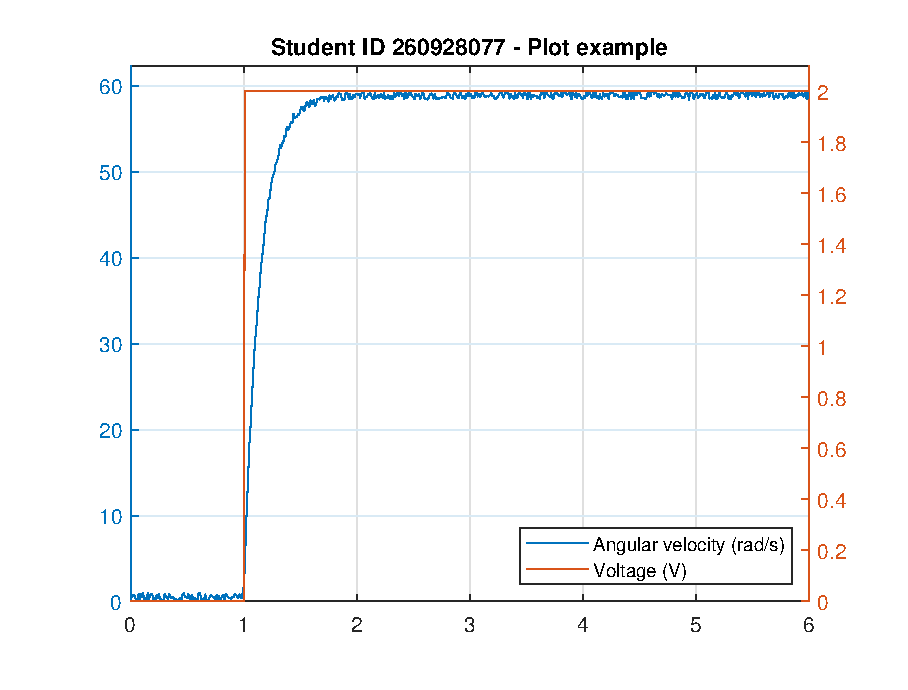
\includegraphics[width=\maxwidth{56.196688409433015em}]{figure_0.eps}
\end{center}


\matlabheading{\textit{2.3. Saving data}}

\begin{par}
\begin{flushleft}
The data generated by the motor can be saved using \texttt{\textbf{Motor.save(...)}}. The \texttt{\textbf{save(...)}} function takes two arguments: the \texttt{\textbf{Students}} structure (that is filled in the beginning of the lab), and a tag to identify data.
\end{flushleft}
\end{par}

\begin{par}
\begin{flushleft}
For example, to save the data from the last experiment with the tag 'Lab03\_example', use:
\end{flushleft}
\end{par}

\begin{matlabcode}
Motor.save(Students, 'Lab03_example');
\end{matlabcode}


\begin{par}
\begin{flushleft}
The data is saved in a \texttt{MAT}-file. In most hardware labs, you will be required to submit the \texttt{MAT} file along with the final LiveScript and the PDF report.
\end{flushleft}
\end{par}

\matlabheading{\textit{2.4. Loading data}}

\begin{par}
\begin{flushleft}
The \texttt{\textbf{Motor.load(...)}} function loads the data saved in the \texttt{MAT}-file. This is useful if your work is lost or corrupted. You can simply load the saved data rather than repeating the experiment. The \texttt{\textbf{load}} function takes 1 argument which is the tag of the data.
\end{flushleft}
\end{par}

\begin{par}
\begin{flushleft}
For example, we can load and plot the previously saved data by:
\end{flushleft}
\end{par}

\begin{matlabcode}
Motor.load('Lab03_example');
\end{matlabcode}
\begin{matlaboutput}
VirtualMotor::load::info: Recovering data collected by students: [260928077] .
\end{matlaboutput}
\begin{matlabcode}

t = Motor.time;
w = Motor.velocity;
v = Motor.voltage;

figure; clf;
yyaxis left
plot(t, w)
ylim([0, 1.05 * max(w)])
yyaxis right
plot(t, v)
ylim([0, 1.05 * max(v)])
xlim([0, startTime + duration])
legend('Angular velocity (rad/s)', 'Voltage (V)', ...
    'location', 'southeast');
title(sprintf('Student ID %s - Plot example', Students.ID));
grid on
\end{matlabcode}
\begin{center}
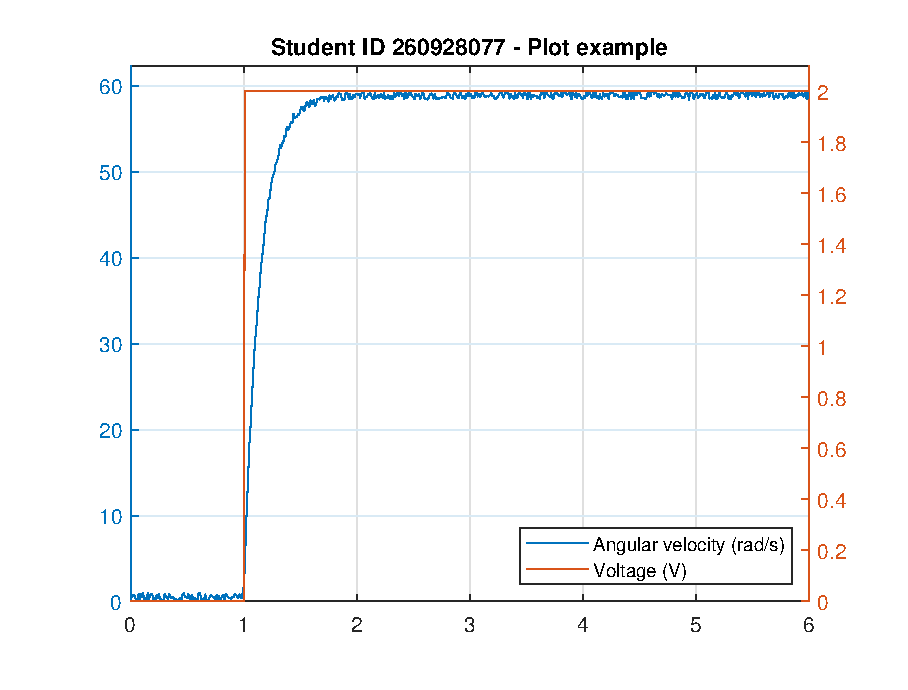
\includegraphics[width=\maxwidth{56.196688409433015em}]{figure_1.eps}
\end{center}


\matlabheading{\textbf{3. Data Collection: Determining Step Response}}

\begin{par}
\begin{flushleft}
The purpose of this experiment is to obtain the step response of the Virtual DC Motor. For this we will send a fixed voltage signal $V_{in} =6$ volts and measure the angular velocity $\Omega$.
\end{flushleft}
\end{par}

\begin{par}
\begin{flushleft}
However, because of static friction, the transfer function between voltage and angular velocity is non linear at small voltages. To avoid this problem, we will apply a constant reference voltage of $V_{ref} =4$ volts, before collecting the step input response.
\end{flushleft}
\end{par}

\matlabheading{\textit{Question 1 (2 marks)}}

\begin{par}
\begin{flushleft}
Complete the code below to apply a reference voltage of 4V for 5 seconds followed by an additional voltage of 6V for 5 seconds.
\end{flushleft}
\end{par}

\begin{matlabcode}
Vref = 4 % Reference signal
\end{matlabcode}
\begin{matlaboutput}
Vref = 4
\end{matlaboutput}
\begin{matlabcode}
Tref = 5 % Duration of reference signal
\end{matlabcode}
\begin{matlaboutput}
Tref = 5
\end{matlaboutput}
\begin{matlabcode}
Vin = 6 % Input signal
\end{matlabcode}
\begin{matlaboutput}
Vin = 6
\end{matlaboutput}
\begin{matlabcode}
Tin = 5 % Duration of input signal
\end{matlabcode}
\begin{matlaboutput}
Tin = 5
\end{matlaboutput}
\begin{matlabcode}

%Reset the motor power and timer
Motor.reset();

% Wait for the starting time (4V for 5s)
Motor.wait(Tref);
Motor.input(Vref);

% Drive the Motor (6V for 5s)
Motor.wait(Tin);
Motor.input(Vin);

% Stop the motor
Motor.off();

Motor.save(Students, 'Lab03.Q1');
\end{matlabcode}


\matlabheading{\textit{Question 2 (1 mark)}}

\begin{par}
\begin{flushleft}
Complete the code below to plot your data
\end{flushleft}
\end{par}

\begin{matlabcode}
t = Motor.time;
w = Motor.velocity;
v = Motor.voltage;


figure; clf;
subplot(2, 1, 1);
% [Answer here] plot angular velocity (w) vs time (t)
plot(t, w)
ylim([100, 180])
xlim([Tref - 1, Tref + Tin])
legend('Angular velocity (rad/s)', 'location', 'best');
title(sprintf('Student ID %s - Question 2 - Data', Students.ID));
grid on
subplot(2, 1, 2)
% [Answer here] plot voltage (v) vs time (t)
plot(t, v)
ylim([3, 7])
xlim([Tref - 1, Tref + Tin])
legend('Voltage (V)', 'location', 'southeast');
grid on
\end{matlabcode}
\begin{center}
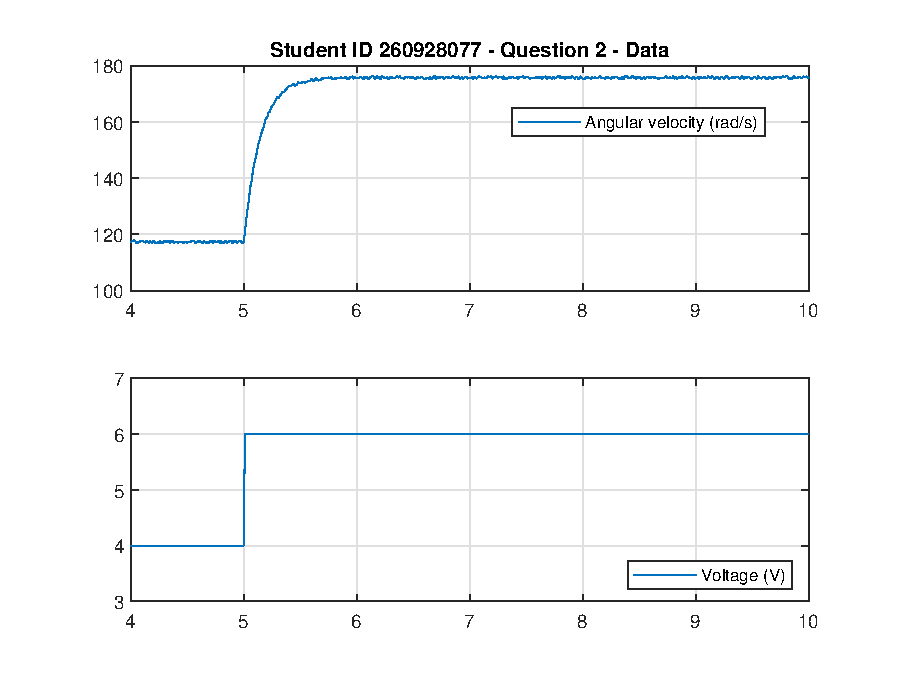
\includegraphics[width=\maxwidth{56.196688409433015em}]{figure_2.eps}
\end{center}


\matlabheading{\textbf{2. System identification}}

\matlabheading{\textit{2.1. Data analysis}}

\begin{par}
\begin{flushleft}
In this section, we will use the step response obtained in \texttt{Question 2} to deduce the DC gain $K$ and the time constant $\tau$. Note that the values shown in a figure can be read by opening the figure and hovering the mouse at top of the line plot.
\end{flushleft}
\end{par}

\begin{par}
\begin{flushleft}
Observe that the measurement of the angular velocity is noisy. The noise can be reduced by taking the approximate average value rather than the exact value.
\end{flushleft}
\end{par}

\begin{par}
\begin{flushleft}
For example, we can get a better approximation of the reference angular velocity $\Omega_{ref}$ resulting from $V_{ref}$ by doing:
\end{flushleft}
\end{par}

\begin{matlabcode}
Wref = mean(w(t > Tref-1 & t < Tref)); % Compute the average value of "w" for "t" between "Tref - 1" and "Tref".
\end{matlabcode}


\matlabheading{\textit{Question 3 (3 marks)}}

\begin{par}
\begin{flushleft}
From the plot in \texttt{Question 2} find the values of DC gain $K$ and time constant $\tau$.
\end{flushleft}
\end{par}

\begin{matlabcode}
% Computer the average value of "w" for t between 9 and 10 
finalValue = mean(w(t > Tref+Tin-1 & t < Tref+Tin));

K = (finalValue - w(t == Tref))/(Vin-Vref)
\end{matlabcode}
\begin{matlaboutput}
K = 29.1576
\end{matlaboutput}
\begin{matlabcode}

% We have to find the corresponding time value 
% (x-axis value) corresponding to the following w
% (y-axis value):
w_corresponding_to_tau = (finalValue- w(t == Tref))*(1- exp(-1)) + w(t == Tref);

% Find the corresponding time (x-axis) value 
% to the above w value (y-axis).
% This is done with 1D interpolation 
tau = interp1(w, t, w_corresponding_to_tau) - Tref
\end{matlabcode}
\begin{matlaboutput}
tau = 0.1450
\end{matlaboutput}


\matlabheading{\textit{2.2. Validating identified system}}

\begin{par}
\begin{flushleft}
We can use \texttt{\textbf{MATLAB}} to validate the calculated values of the DC gain and time constant. For this we will simulate a first order system with those values and compare it to the experimental results.
\end{flushleft}
\end{par}

\matlabheading{\textit{Question 4 (1 mark)}}

\begin{par}
\begin{flushleft}
Define a first order transfer function with the DC gain and time constant that you have obtained (use \texttt{\textbf{tf}} or \texttt{\textbf{zpk}})
\end{flushleft}
\end{par}

\begin{matlabcode}
s = tf('s');

H = (K/(tau*s+1))
\end{matlabcode}
\begin{matlaboutput}
H =
 
     29.16
  -----------
  0.145 s + 1
 
Continuous-time transfer function.
\end{matlaboutput}


\begin{par}
\begin{flushleft}
The following code simulates the transfer function H(s) with a 2 volts input starting at $T_{ref}$. We are using \texttt{\textbf{MATLAB}} function \texttt{\textbf{lsim}} to simulate the output of a linear system with a given input.
\end{flushleft}
\end{par}

\begin{matlabcode}
tSim = t(t >= Tref & t < Tref+Tin) - Tref; % create a time signal from Tref to Tref + Tin
vSim = (Vin - Vref) * ones(size(tSim)); % create a constant voltage of Vin-Vref = 2 volts
vSim(1) = 0; % the initial state of the system is zero
wSim = Wref + lsim(H, vSim, tSim); % simulate the output of the system H
\end{matlabcode}


\begin{par}
\begin{flushleft}
The following code shows the simulation and the experimental results on the same plot.
\end{flushleft}
\end{par}

\begin{matlabcode}
figure; clf;
hold on
plot(t, w) % experimental results
plot(tSim+Tref, wSim, 'r') % simulation of the identified transfer function
ylim([100, 180])
xlim([Tref - 1, Tref + Tin])
legend('Angular velocity (rad/s)', ...
    'Simulated angular velocity (rad/s)', ...
    'location', 'southeast');
title(sprintf('Student ID %s - Identification of Virtual DC Motor', Students.ID));
grid on
\end{matlabcode}
\begin{center}
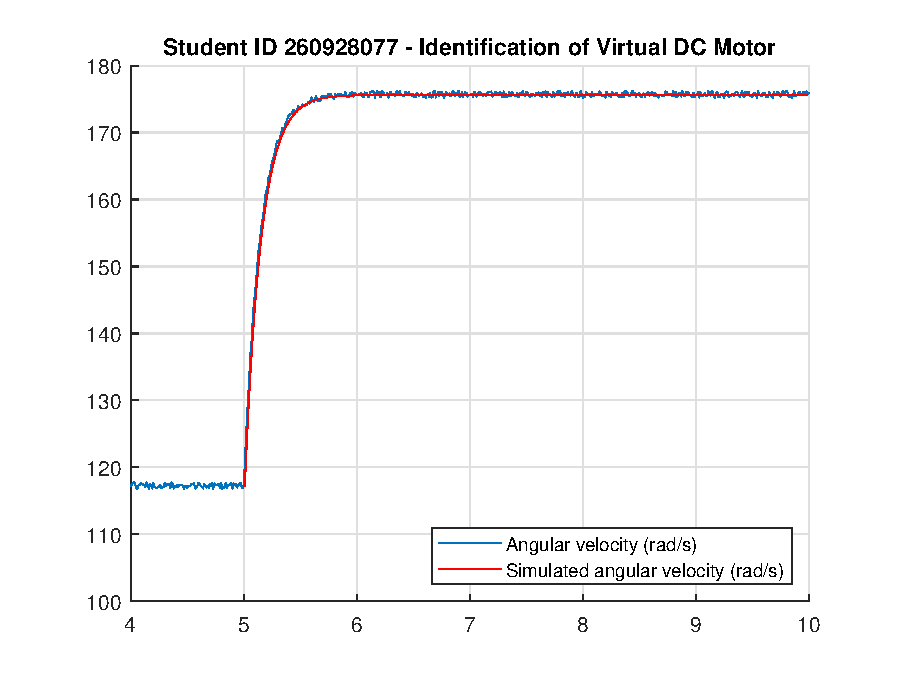
\includegraphics[width=\maxwidth{56.196688409433015em}]{figure_3.eps}
\end{center}


\begin{par}
\begin{flushleft}
We can measure the goodness of fit of the transfer function prediction by computing the Root-mean-square error (RMSE) between the experimental data and the predicted angular velocity with the model.
\end{flushleft}
\end{par}

\begin{par}
$$RMSE=\sqrt{{{\frac{\sum_{i=1}^n (\omega_{Sim} (i)-\omega_{Exp} (i))^2 }{n}}}}$$
\end{par}

\begin{par}
\begin{flushleft}
where $n$ is the number of elements in the angular velocity signal.
\end{flushleft}
\end{par}

\matlabheading{\textit{Question 5 (2 marks)}}

\begin{itemize}
\setlength{\itemsep}{-1ex}
   \item{\begin{flushleft} Complete the code to compute the RMSE of your fit \end{flushleft}}
\end{itemize}

\begin{matlabcode}
wExp = w(t >= Tref & t < Tref+Tin); % get the values of w between Tref and Tref + Tin


% note: length(wExp) = length(wSim)

sumResult = 0;
for i=1 : length(wSim)
    sumResult = sumResult + (wSim(i)-wExp(i)).^2;
end
sumResult;

RMSE = sqrt(sumResult/length(wExp))
\end{matlabcode}
\begin{matlaboutput}
RMSE = 0.5755
\end{matlaboutput}


\begin{itemize}
\setlength{\itemsep}{-1ex}
   \item{\begin{flushleft} Can you tweak the values of the DC gain $K$ and time constant $\tau$ to get a better fit of the experimental data? Complete the following code to change the values of $K_{new}$ and $\tau_{new}$, re-define the transfer function $H_{new}$, re-simulate the new angular velocity, re-calculate the new RMSE, and re-plot the new fit. \end{flushleft}}
\end{itemize}

\begin{matlabcode}
KNew = K + 0.08
\end{matlabcode}
\begin{matlaboutput}
KNew = 29.2376
\end{matlaboutput}
\begin{matlabcode}
tauNew = tau - 0.01
\end{matlabcode}
\begin{matlaboutput}
tauNew = 0.1350
\end{matlaboutput}
\begin{matlabcode}
HNew = (KNew/(tauNew*s+1))
\end{matlabcode}
\begin{matlaboutput}
HNew =
 
     29.24
  -----------
  0.135 s + 1
 
Continuous-time transfer function.
\end{matlaboutput}
\begin{matlabcode}

wSimNew = Wref + lsim(HNew, vSim, tSim);


sumResultNew = 0;
for i=1 : length(wSimNew)
    sumResultNew = sumResultNew + (wSimNew(i)-wExp(i)).^2;
end
sumResultNew;

RMSENew = sqrt(sumResultNew/length(wExp))
\end{matlabcode}
\begin{matlaboutput}
RMSENew = 0.4284
\end{matlaboutput}
\begin{matlabcode}



figure; clf;
hold on
plot(t, w) % experimental results
plot(tSim+Tref, wSimNew, 'r') % simulation of the identified transfer function
ylim([100, 180])
xlim([Tref - 1, Tref + Tin])
legend('Angular velocity (rad/s)', ...
    'Simulated angular velocity (rad/s)', ...
    'location', 'southeast');
title(sprintf('Student ID %s - Question 5 - New RMSE = %4.2f', Students.ID, RMSENew));
grid on
\end{matlabcode}
\begin{center}
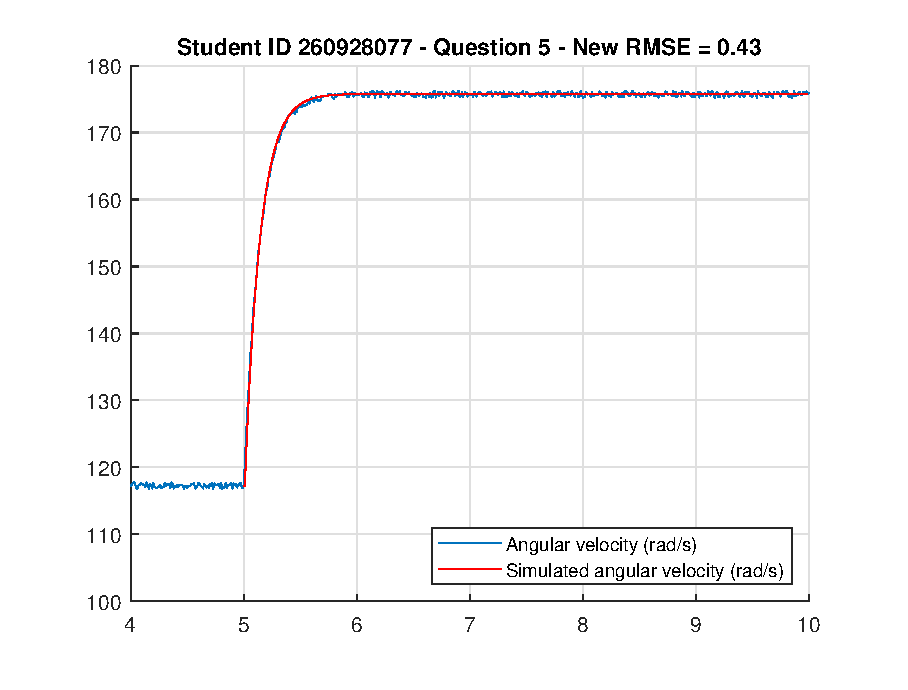
\includegraphics[width=\maxwidth{56.196688409433015em}]{figure_4.eps}
\end{center}
\begin{matlabcode}


% While playing with different value of KNew and tauNew we ralize that 
% any change in taoNew will affect the time the signal takes to reach its
% maximum and a change in k will change the maximum value reached by the
% signal. We can therefore conclude that the simulation done in previous
% question is the closest simulation possible 

% Note we still can add/substract very small values to decrease the RMSE by
% a small amount (like what we did above with Knew and taoNew) but that
% shouldn't affect the above mentioned conclusion 
\end{matlabcode}


\matlabheading{\textit{Question 6 (1 mark)}}

\begin{par}
\begin{flushleft}
Another way to write the transfer function of a DC motor is as follows: $H(s)={{\frac{K_t }{JRs+bR+K_t K_e }}}$
\end{flushleft}
\end{par}

\begin{par}
\begin{flushleft}
Where
\end{flushleft}
\end{par}

\begin{itemize}
\setlength{\itemsep}{-1ex}
   \item{\begin{flushleft} $K_t$ is the torque proportionality constant in (Kg $m^2$/ $s^2$/A) or (N m/A) \end{flushleft}}
   \item{\begin{flushleft} $K_e$ is the back electromotive proportionality constant in (V/rad/s) \end{flushleft}}
   \item{\begin{flushleft} $R$ is the terminal resistance (Ohm) \end{flushleft}}
   \item{\begin{flushleft} $J$ is the motor inertia (kg $m^2$) \end{flushleft}}
   \item{\begin{flushleft} $b$ is the motor viscous friction constant in (Kg $m^2$/s) or (N m s) \end{flushleft}}
\end{itemize}

\begin{par}
\begin{flushleft}
Suppose we know that
\end{flushleft}
\end{par}

\begin{matlabcode}
Kt = 0.034;
Ke = 0.034;
R = 8.4;
\end{matlabcode}


\begin{par}
\begin{flushleft}
Using the information obtained earlier, calculate the Motor viscous friction constant $b$.
\end{flushleft}
\end{par}

\begin{matlabcode}
% Comparing the transfer function from previous questions and 
% The DC motor transfer function we find: 

cons = K/Kt;
% cons(bR+Kt*Ke) = 1
% Kt*Ke+bR = 1/cons
% bR = 1/cons - Kt*Ke
b = (1/cons - Kt*Ke)/R
\end{matlabcode}
\begin{matlaboutput}
b = 1.1995e-06
\end{matlaboutput}
\begin{matlabcode}

\end{matlabcode}

\end{document}
